\section{Vektorräume}
In diesem Kapitel sei $ \K $ ein beliebiger Körper.

\subsection{Vektorraum (VR)}
\subsubsection{$ \K^n $ und $ \K^X $}
Sei $ n \in \N $. Die Menge $ \K^n $ wird
\begin{align*}
	& \text{mit der Addition} & + &: \K^n \times \K^n \to \K^n\\
	& \text{und der Skalarmultiplikation} & \cdot &: \K \times \K^n \to \K^n
\end{align*}
ausgestattet, die durch 
\begin{align*}
	(x_1, \ldots, x_n) + (y_1, \ldots, y_n) &:= (x_1+y_1, \ldots, x_n+y_n)\\
	\alpha (x_1, \ldots, x_n) &:= (\alpha x_1, \ldots,\alpha x_n)
\end{align*}
für alle $ (x_1, \ldots, x_n), (y_1, \ldots, y_n) \in \K^n $ und alle $ \alpha \in \K $ definiert sind.\\[10pt]
Sei $ X $ nichtleere Menge ($ X $ kann unendlich sein). % $ X $ oder $ |X| $?
Wir definieren in $ \K^X $ $ + : \K^X \times \K^X \to \K^X $ und $ \cdot : \K \times \K^X \to \K^X $ durch:
\begin{align*}
	(f+g)(x) &:= f(x) + g(x) \\
	(\alpha \cdot f) (x) &:= \alpha \cdot f(x)
\end{align*}

TODO: Bild mit Vektoren $u=(3,1)$, $v=(1,2)$, $u+v$, $2 u$ und $-v$. 

\begin{bsp} 
$\K^X$ benutzt man unter anderem in Kontexten, bei denen man die Variablen nicht mit Nummern sondern mit anderen Labels versehen will, in $\R^X$ mit $X = \{ CHF, CNY, EUR, GBP \}$ kann man etwa den Vektor $v \in \R^X$ der aktuellen Währungskurse Betrachten mit $v(CHF)=1{.}10, \ v(CNY)=0{.}15, \ v(EUR) = 1{.}19, \ v(GBP) = 1{.}34$. Solche Kontexte sind zum Beispiel in der kombinatorischen Optimierung reichlich vorhanden. Natürlich kann man in diesem Beispiel die Variablen nummerieren und mit $\R^4$ an der Stelle von $\R^X$ arbeiten. 
\end{bsp} 

\subsubsection{Vektorraum über $ \K $}

Abstrakt definierte Vektorräume geben einem einen konzeptuellen Zugang zur Theorie der Vektorräume, ohne dass man in konkreten Situationen an die Koordinaten (wie bei $\K^n$) denken muss. 

Eine Menge $ V $ mit Addition $ + : V \times V \to V  $ und Skalarmultiplikation $ \cdot : \K \times V \to V $ heißt Vektorraum über $ \K $, falls:

\setlength{\myindent}{
	\maxof{
		\widthof{(V1)}
	}{
		\widthof{(V2)}
	}
}
\advance\myindent by \the\labelsep

\begin{itemize}[leftmargin=\myindent]
	\item[(V1)]
		$ (V,+) $ ist abelsche Gruppe
	\item[(V2)]
		$ \begin{aligned}[t]
			(\lambda + \mu)v &= \lambda v + \mu v & \\
			\lambda (v + w) &= \lambda v + \lambda w \\
			(\lambda \cdot \mu) \cdot v &= \lambda \cdot (\mu \cdot v) \\
			1 \cdot v &= v
		\end{aligned} $
		für alle $\lambda, \mu \in \K$ und $v, w\in V$
\end{itemize}

Kurze Erinnerung an abelsche Gruppen: da hat man eine $0$, zu jedem $u$ findet man das $-u$, und $+$ ist kommutativ und assoziativ. 


\begin{bem}[Begriffe / Bezeichnungen]\
\begin{itemize}
	\item
		$ 0 \in V $ heißt Nullvektor $ (0, \ldots, 0) $.
	\item
		Elemente von $ V $ heißen Vektoren
	\item
		Elemente von $ \K $ heißen Skalare
	\item
		$ \cdot $ wird oft in Formeln weggelassen ($ \cdot $ höhere Priorität als $ + $)
\end{itemize}
\end{bem}

\begin{propn}
	Sei $ V $ Vektorraum über $ \K $. Sei $ \lambda \in \K $ und $ v \in V $, dann:
	\begin{enumerate}
		\item
			$ \lambda \cdot v = 0 \Leftrightarrow  \lambda = 0 $ oder $ v=0 $
		\item
			$ (-1) \cdot v = -v $
	\end{enumerate}
\end{propn}
\begin{proof}
	Übungsaufgabe.
\end{proof}

\clearpage
\subsection{Untervektorräume (UVR)}
\subsubsection{Untervektorraum}

Sei $ V $ Vektorraum über $ \K $ und sei $ W \subseteq V $. Dann heißt $ W $ Untervektorraum von $ V $, wenn:

\setlength{\myindent}{
	\maxof{
		\widthof{(UV1)}
	}{
		\maxof{
			\widthof{(UV2)}
		}{
			\widthof{(UV3)}
		}
	}
}
\advance\myindent by \the\labelsep

\begin{itemize}[leftmargin=\myindent]
	\item[(UV1)]
		$ W \neq 0 $
	\item[(UV2)]
		$ v,w \in W \Rightarrow v+w \in W $
	\item[(UV3)]
		$ \alpha \in \K, v \in W \Rightarrow \alpha \cdot v \in W $
\end{itemize}

\begin{bem}
Ein LGS, dessen alle rechten Seiten gleich $0$ sind, nennt man homogen. Die Lösungsmenge eines LGS in $n$ Variablen ist ein UVR von $\K^n$. 
\end{bem}

\begin{bsp}
	Sei $\K = \Z/ 2 \Z = \{0,1\}$. In der Codierungstheorie heißen die UVR von $\K^n$ binäre lineare Codes der Länge $n$. Die Lösungsmenge 
	\begin{align*}
		W & = \{ (x_1,x_2,x_3) \in \K^3 \,:\, x_1 + x_2 + x_3 = 0 \}
		\\ & = \{ (0,0,0), (1,0,1), (0,1,0), (1,1,0) \}. 
	\end{align*}
	der homogenen Gleichung $x_1 + x_2 + x_3=0$ 
	ist etwa ein binärer linearer Code der Länge $3$. Bei einer digitalen Kommunikation mit der Verwendung von $W$, kann man zwei Bits $(a,b) \in \K^2$ als den Code $x=(a, b, a+b) \in W$ verschicken. Empfängt man infolge einer Störung nicht $x$ sondern einen anderen Vektor $y \in \K^3$, der nicht zu $W$ gehört, so weiß man, dass während der Übertragung ein Fehler aufgetreten ist. Durch unser Beispiel-Code $W$ kann $y$ nicht zu $x$ korrigiert werden, es gibt aber andere Codes, mit denen man eine gewisse Anzahl an Fehlern in $y$ korrigieren kann. 
\end{bsp} 

\begin{bsp}
	In Machine Learning und Statistik können Abhängigkeiten in einer Datenmenge $u_1,\ldots, u_N \in \R^n$ mit Hilfe von Untervektorräumen von $U$ von $\R^n$ beschrieben. Mehr dazu später? TODO: Ein Bild für $n=2$. Stichpunkt: lineare Regression. Hierzu gibt es zahlreiche Anwendungsmöglichkeiten (Abhängigkeiten in Kundenbewertungen bei Netflix, Amazon usw.)
\end{bsp} 


\subsubsection{Kriterium für Untervektorräume}
\begin{thm}
	Sei $ V $ Vektorraum über $ \K $ und sei $ W \subseteq V $. Dann sind die folgenden Bedingungen äquivalent:
	\begin{enumerate}
		\item
			$ W $ ist Untervektorraum von $ V $
		\item
			$ + $ und $ \cdot $ lassen sich von $ V $ auf $ W $ einschränken und darüber hinaus ist $ W $ Vektorraum über $ \K $ bezüglich dieser Operationen.
	\end{enumerate}
\end{thm}
\begin{proof}
	Folgt direkt aus der Definition.
\end{proof}

\subsubsection{Durchschnitt von Untervektorräumen}
\begin{propn}
	Sei $ V $ Vektorraum über $ \K $. Sei $ I $ nichtleere Menge und sei $ W_i $ Untervektorraum von $ V $ für jedes $ i \in I $. Dann ist auch
	\begin{equation*}
		W := \bigcap_{i \in I} W_i
	\end{equation*}
	ein Untervektorraum von $ V $. % @Phil: So richtig?
\end{propn}
\begin{proof}
	Erst $ 0 \in W $ nachweisen, der Rest folgt direkt.
\end{proof}

\subsubsection{Vereinigung von Untervektorräumen}
\begin{propn}
	Sei $ V $ Vektorraum über $ \K $. Seien $ W $ und $ W' $ Untervektorräume von $ V $ derart, dass $ W \cup W' $ auch ein Untervektorraum von $ V $ ist. Dann gilt
	\begin{equation*}
		W \subseteq W' \text{ oder } W' \subseteq W.
	\end{equation*}
\end{propn}
\begin{proof}
	Wir nehmen $ W \not\subseteq W' $ an und zeigen $ W' \subseteq W $. Fixiere $ w \in W \setminus W' $. Sei $ w' \in W' $ beliebig. Zu zeigen: $ w' \in W $.
	
	Da $ W \cup W' $ Untervektorraum ist, folgt aus $ w,w' \in W \cup W' $, dass $ w + w' \in W \cup W' $. Es gilt $ w + w' \in W \setminus W' $, denn sonst $ w+w' \in W' \Rightarrow w = \underbrace{\left( w+w' \right)}_{ \in W'} - \underbrace{\vphantom{\left( w' \right)} w'}_{\in W'} \in W' $ ($ \Rightarrow \lightning $ zur Wahl von $ w \in W \setminus W' $).

	Es folgt $ w+w' \in W \Rightarrow w, w+w' \in W $ und weil $ W $ Untervektorraum ist, gilt $ w' = \underbrace{(w+w')}_{\in W} - \underbrace{\vphantom{\left( w' \right)} w}_{\in W} \in W $.
\end{proof}

\subsection{Linearkombinationen}
\subsubsection{Linearkombination}
Sei $ r \in \N_0 $ und seien $ v_1, \ldots, v_r $ Vektoren in einem Vektorraum $ V $ über $ \K $. Seien  $ \lambda_1, \ldots, $ $ \lambda_r \in \K $. Dann heißen $ \lambda_1 v_1 + \ldots + \lambda_r v_r $ die Linearkombination von $ v_1, \ldots, v_r $ mit Koeffizienten $ \lambda_1, \ldots, \lambda_r $.
	
Im Fall $ r = 0 $ setzt man die Linearkombination gleich $ 0 \in V $. Sei $ I $ Menge und $ v_i \in V $ für jedes $ i \in I $ Dann heißt
\begin{equation}
	\lin_\K (v_i)_{i \in I} := \{ \lambda_1 v_{i_1} + \ldots + \lambda_r v_{i_r} : \lambda_1, \ldots, \lambda_r \in \K, i_1, \ldots, i_r \in I, r \in \N_0 \}
\end{equation}  
die \emph{lineare Hülle} von $ (v_i)_{i \in I} $. Insbesondere gilt
\begin{equation}
	\lin_\K (v_1, \ldots, v_r) := \{ \lambda_1 v_1 + \ldots + \lambda_r v_r : \lambda_1, \ldots, \lambda_r \in \K \}.
\end{equation}
Hier und im folgenden: wenn die Wahl des Index $ \K $ klar ist, wird der Index weg gelassen.

Man kann auch von der linearen Hülle einer Menge $ M \subseteq V $ reden:
\begin{equation}
\lin(M) := \{ \lambda_1 v_1 + \ldots + \lambda_r v_r : \lambda_1, \ldots, \lambda_r \in \K, v_1, \ldots, v_r \in M, r \in \N_0 \}
\end{equation}


\begin{propn}
	Sei $ V $ Vektorraum über $ \K $. Sei $ I $ Menge und sei $ v_i \in V $ für jedes $ i \in I $. Dann gilt:
	\begin{itemize}
		\item[(a)]
			$ \lin (v_i)_{i \in I} $ ist Untervektorraum von $ V $.
		\item[(b)]
			Ist $ W $ Untervektorraum von $ V $ mit $ v_i \in W $ für alle $ i \in I $, dann ist $ \lin (v_i)_{i \in I} \subseteq W $.
	\end{itemize}
\end{propn}
\begin{proof}
	Direkt.
\end{proof}


\begin{bsp} Beispiele für $ \mathbb{R}^3 $
\begin{itemize}
	\item
		$ \lin (v) $ mit $ v \neq 0 $ ist eine Gerade durch $ 0 $.
	\item
		$ \lin (v,w) $ mit $ v \neq 0 $ und $ w \notin \lin(v) $ ist eine Ebene durch $ 0 $.
\end{itemize}
\end{bsp} 


\subsubsection{Lineare Unabhängigkeit und Abhängigkeit}

Sei $ r \in \N_0 $ und seien $ v_1, \ldots, v_r $ Vektoren in einem Vektorraum über $ \K $. Die Vektoren $ v_1, \ldots, v_r $ heißen \emph{linear unabhängig}, falls für alle $ \lambda_1, \ldots, \lambda_r \in \K $ aus $ \lambda_1v_1 + \ldots + \lambda_rv_r = 0 $ die Gleichungen $ \lambda_1 = \ldots = \lambda_r = 0 $ folgen.

Sei $ I $ Menge und $ v_i \in V $ für jedes $ i \in I $. Die Vektoren $ v_i $ mit $ i \in I $ heißen linear unabhängig, falls für jede endliche Teilmenge $ J $ von $ I $ die Vektoren $ v_j $ mit $ j \in J $ linear unabhängig sind. Die Vektoren $ v_i $ mit $ i \in I $ heißen \emph{linear abhängig}, falls sie nicht linear unabhängig sind. 

	Vektoren $ v_1, \ldots, v_r \in V $ mit $ r \in \N_0 $ sind genau dann linear abhängig, wenn $ \lambda_1, \ldots, \lambda_r $ mit $ \lambda_1v_1 + \ldots + \lambda_rv_r = 0 $ und $ ( \lambda_1, \ldots, \lambda_r ) \neq ( 0, \ldots, 0 ) $ existieren.

	Ein System aus  Nullvektoren ist linear unabhängig.
	
\begin{bsp}
	Vektoren $v_1= (2,-1,3), v_2 = (1,2,0)$ und $v_3 = (-4,7,-9)$ aus $\R^3$ sind linear abhängig, denn $ 3 v_1 - 2 v_2 + v_3 = (0,0,0)$. Je, zwei der drei Vektoren $v_1, v_2, v_3$ sind aber linear unabhängig. 
\end{bsp} 

\begin{bem}
	Für gegebene $v_1,\ldots,v_r \in \K^n$ ist die Vektorgleichung $\lambda_1 v_1 + \cdots + \lambda_r v_r = 0$, wenn man sie komponentenweise ausschreibt, ein LGS aus $n$ Gleichungen in $r$ Unbekannten $\lambda_1,\ldots,\lambda_r \in \K$. Ob $v_1,\ldots,v_r$ linear (un)abhängig sind kann also mit Hilfe des Gauß-Verfahrens getestet werden. 
\end{bem} 


\subsubsection{Kriterien für lineare Unabhängigkeit}

\begin{thm}
	Sei $ V $ Vektorraum über $ \K $. Sei $ I $ Menge und sei $ v_i \in V $ für jedes $ i \in I $. Dann sind die folgenden Bedingungen äquivalent:
	\begin{enumerate}
		\item Vektoren  $ v_i $ mit $ i \in I $ sind linear unabhängig.
		\item Jedes $ v \in \lin(v_i)_{i \in I} $ lässt sich in eindeutiger Weise als Linearkombination von $ (v_i)_{i \in I} $ darstellen.
	\end{enumerate}
\end{thm}
\begin{proof}\
\begin{description}[font=\normalfont]
	\item[(ii) $ \Rightarrow $ (i):]
	Angenommen, (ii) gilt. Dann lässt sich der Nullvektor in eindeutiger Weise als Linearkombination der Vektoren $ v_i $ mit $ i \in I $. Diese eindeutige Weise ist: alle Koeffizienten = 0. Also sind $ v_i $ mit $ i \in I $ linear unabhängig.

	\item[(i) $ \Rightarrow $ (ii):]
	Angenommen, (i) gilt. Wir zeigen (ii) durch einen Widerspruchsbeweis. Wir nehmen an, (ii) gilt nicht, d.h. für ein $ v \in V $ gilt $ v = \sum_{i \in I} \lambda_iv_i = \sum_{i \in I} \mu_iv_i $, sodass $ \lambda_i, \mu_i \in \K $ und nur endlich viele dieser Skalare von Null verschieden sind, und für mindestens ein $ k \in I $ die Bedingung $ \lambda_k \neq \mu_k $ erfüllt ist.

	Dann $ 0 = v - v = \sum_{i \in I} \lambda_iv_i - \sum_{i \in I} \mu_iv_i = \sum_{i \in I} (\lambda_i - \mu_i)v_i $ mit $ \lambda_k - \mu_k \neq 0 $ für $ k $ wie oben. $ \Rightarrow $ $ (v_i)_{i \in I} $ sind linear abhängig $ \Rightarrow \lightning $ zu (i). \qedhere
\end{description}
\end{proof}

\subsubsection{Eigenschaften der linearen Abhängigkeit}

\begin{propn}
	Sei $ V $ Vektorraum über $ \K $. Dann gilt:
	\begin{enumerate}
		\item Ein einziger Vektor $ v $ ist genau dann linear abhängig, wenn $ v = 0 $.
		\item Gehört $ 0 \in V $ zu einer Familie von Vektoren, so sind diese linear abhängig.
		\item Kommt der gleiche Vektor in einer Familie von Vektoren mehrmals vor, so sind die Vektoren der Familie linear abhängig. 
		\item Für $ r \in \N, r \geq 2 $ sind Vektoren $ v_i, \ldots, v_r \in V $ genau dann linear abhängig, wenn ein $ j \in \{ 1, \ldots, r \} $ existiert mit $ v_j \in \lin \bigl(v_i \bigr)_{i \in \{ 1, \ldots, r \} \setminus \{ j \} } $.
	\end{enumerate}
\end{propn}

\begin{proof} (i), (ii) und (iii) sind klar.
\begin{itemize}
	\item[(iv)]
	Sind $ v_1, \ldots, v_r $ linear abhängig, so gilt $ 0 = \lambda_1v_1 + \ldots + \lambda_rv_r $ mit gewissen $ \lambda_1, \ldots, \lambda_r \in \K $ und mit $ \lambda_k \neq 0 $ für ein $ k \in \{ 1, \ldots, r \} \Rightarrow -\lambda_kv_k = \sum_{i \in \{ 1, \ldots, r \} \setminus \{ k \}} \lambda_iv_i \Rightarrow v_k = \sum_{i \in \{ 1, \ldots, r \} \setminus \{ k \}} - \frac{\lambda_i}{\lambda_k}v_i $.
	
	Umgekehrt: wenn $ v_k \in lin(v_i)_{i \in \{ 1, \ldots, r \} \setminus \{ k \}} $, d.h. $ v_k = \sum_{i \in \{ 1, \ldots, r \} \setminus \{ k \}} \lambda_iv_i $ mit $ \lambda_i \in \K $ für alle $ i \in \{ 1, \ldots, r \} \setminus \{ k \} $, so kann man $ \lambda_k := -1 $ setzen und erhält $ 0 = \sum_{i = 1}^r \lambda_iv_i $ mit $ ( \lambda_1, \ldots, \lambda_r ) \neq ( 0, \ldots, 0 ) $. Also sind $ v_1, \ldots, v_r $ linear abhängig. \qedhere
\end{itemize}
\end{proof}

\subsection{Basis und Dimension}

\subsubsection{Erzeugendensysteme und Basen}

Sei $ I $ Menge und seien $ v_i $ mit $ i \in I $ Vektoren aus einem VR $ V $ über $ \K $. Dann heißt die Familie $ (v_i)_{i \in I} $ \emph{Erzeugendensystem} von $ V $, falls $ \lin(v_i)_{i \in I} = V $.

Die Familie $ (v_i)_{i \in I} $ heißt \emph{Basis} von $ V $, falls $ (v_i)_{i \in I} $ ein linear unabhängiges Erzeugendensystem von $ V $ ist. Ist $ (v_i)_{i \in I} $ Basis und $ I $ eine endliche Menge, so heißt $ |I| $ die Länge der Basis $ (v_i)_{i \in I} $.

Ein VR $ V $ heißt \emph{endlich erzeugt}, falls $ V $ eine endliche Basis besitzt.

\subsubsection{Charakterisierungen der Basis-Eigenschaft und die Folgerungen daraus}

\begin{thm}
	Sei $ V $ Vektorraum über $ \K $, sei $ n \in \N $ und $ v_1, \ldots, v_n \in V $. Dann sind die folgenden Bedingungen äquivalent:
	\begin{enumerate}[label=\normalfont(\roman*)]
		\item $ v_1, \ldots, v_n $ bilden eine Basis.
		\item $ \lin(v_1, \ldots, v_n) = V $ und $ V \neq \lin(v_i)_{i \in \{ 1, \ldots, n \} \setminus \{ r \}} $ für alle $ r \in \is{1}{n} $.
		\item Zu jedem $ v \in V $ gibt es eindeutige $ \lambda_1, \ldots, \lambda_n \in \K $ mit $ v = \lambda_1v_1 + \ldots + \lambda_nv_n $.
		\item $ v_1, \ldots, v_n $ sind linear unabhängig und für jedes $ v \in V $ sind $ v_1, \ldots, v_n, v $ linear abhängig.
	\end{enumerate}
\end{thm}
\begin{proof}
\begin{description}[font=\normalfont]
	\item[(i) $ \Rightarrow $ (ii):]
	Sei (i) erfüllt. Angenommen, (ii) wäre nicht erfüllt. Dann gilt $ v_r := \sum_{i \in \{ 1, \ldots, n \} \setminus \{ r \}} \lambda_iv_i $ für ein $ r \in \{ 1, \ldots, n \} $ und gewisse $ \lambda_i \in \K $ mit $ i \in \{ 1, \ldots, n \} \setminus \{ r \} $. Dann gilt $ 0 = \sum_{i = 1}^n \lambda_iv_i $, wobei $ \lambda_r := -1 $ gesetzt wird. Es gilt $ (\lambda_1, \ldots, \lambda_n) \neq (0, \ldots, 0) $. D.h. $ v_1, \ldots, v_n $ sind linear abhängig, Widerspruch zu (i).
	
	\item[(ii) $ \Rightarrow $ (iii):]
	Sei (ii) erfüllt. Angenommen, (iii) wäre nicht erfüllt. Dann existiert $ v \in V $ derart, dass $ v = \sum_{i=1}^n \lambda_iv_i = \sum_{i=1}^n \mu_iv_i $ mit $ \lambda_1, \ldots, \lambda_n, \mu_1, \ldots, \mu_n \in \K $ und mit $ \lambda_r \neq \mu_r $ für mindestens ein $ r \in \{ 1, \ldots, n \} $. Dann $ 0 = \sum_{i=1}^n (\lambda_i - \mu_i)v_i \Rightarrow 0 = \sum_{i=1}^n \frac{\lambda_i - \mu_i}{\lambda_r - \mu_r}v_i \Rightarrow v_r = \sum_{i \in \{ 1, \ldots, n \} \setminus \{ r \}} \frac{\lambda_i - \mu_i}{\lambda_r - \mu_r}v_i \Rightarrow v_r \in \lin(v_i)_{i \in \{ 1, \ldots, n \} \setminus \{ r \}} \Rightarrow$ Widerspruch zu (ii).
	
	\item[(iii) $ \Rightarrow $ (iv):]
	Angenommen, (iii) gilt. Zu zeigen: (iv). Anwendung von (iii) für den Fall $ v = 0 $ ergibt die lineare Unabhängigkeit von $ v_i, \ldots, v_n $. Sei $ v \in V $ beliebig. Nach (iii) existieren $ \lambda_1, \ldots, \lambda_r \in \K $ mit $ v = \sum_{i=1}^r \lambda_iv_i \Rightarrow \lambda_1v_1 + \ldots + \lambda_rv_r + (-1)v = 0 $, wobei $ \lambda_i \neq 0 $. D.h. $ v_1, \ldots, v_r, v $ sind linear abhängig.
	
	\item[(iv) $ \Rightarrow $ (i):]
	Angenommen, (iv) gilt. Wir zeigen (i). Es muss gezeigt werden, dass $ V = \lin(v_1, \ldots, v_n) $ gilt. Sei $ v \in V $ beliebig. Wegen (iv) sind $ v_1, \ldots, v_n, v $ linear abhängig. D.h. $ \lambda_1v_1 + \lambda_nv_n + \lambda v = 0 $ für gewisse $ \lambda_1, \ldots, \lambda_n, \lambda \in \K $ mit $ \lambda_i \neq 0 $. Es gilt $ \lambda \neq 0 $, denn sonst wären $ v_1, \ldots, v_n $ linear abhängig, was der Bedingung (iv) widerspricht. Es folgt $ v = \sum_{i=1}^n \frac{\lambda_i}{\lambda}v_i \in \lin(v_1, \ldots, v_n) $. \qedhere
\end{description}
\end{proof}

%19.11.2014
\begin{klr}
	Sei $ V $ ein Vektorraum über $ \K $, der \emph{nicht} endlich erzeugt ist. Dann besitzt $ V $ ein unendliches System von linear unabhängigen Vektoren.
\end{klr}
\begin{proof}
	Ein System aus Vektoren $ v_1, \ldots, v_n \in V $ mit $ n = 0 $ ist linear unabhängig. Für ein beliebiges linear unabhängiges System $ v_1, \ldots, v_n \in V $ mit $ n \in \N_0 $ kann man ein $ v \in V $ finden, sodass die $ n+1 $ Vektoren $ v_1, \ldots, v_n, v $ linear unabhängig sind. Denn sonst wäre $ v_1, \ldots, v_n $ nach dem vorigen Theorem eine Basis und dadurch der Raum $ V $ endlich erzeugt.
	
	Das iterative Anwenden der vorigen Prozeduren ergibt ein unendliches System von linear unabhängigen Vektoren.
\end{proof}

\subsubsection{Basisauswahlsatz}

\begin{thm}
	Sei $ V $ ein endlich erzeugter Vektorraum über $ \K $. Dann besitzt $ V $ eine Basis.
\end{thm}
\begin{proof}
	Sei $ v_1, \ldots, v_m $ mit $ m \in \N_0 $ ein System von Vektoren aus $ V $, die $ V $ erzeugen. Wenn man in $ \{ v_1, \ldots, v_m \} $ ein $ v_i $ findet ($ i \in \{ 1, \ldots, m \} $), sodass $ v_i \in \lin(v_j)_{j \in \{ 1, \ldots, m \}\setminus\{ i \}} $, dann ersetzt man $ v_1, \ldots, v_m $ durch $ \lin(v_j)_{j \in \{ 1, \ldots, m \}\setminus\{ i \}} $. Nach dieser Änderung bleibt das System erzeugend.
	
	Man wiederholt den vorigen Schritt solange, bis $ v_i \not\in \lin(v_j)_{j \in \{ 1, \ldots, m \}\setminus\{ i \}} $ für alle $ i \in \{ 1, \ldots, m \} $ gilt. Nach Theorem 3.4.2 ist $ v_1, \ldots, v_m $ mit den vorigen Eigenschaften eine Basis.
\end{proof}

\subsubsection{Austauschlemma}

\begin{lm}
	Sei $ V $ Vektorraum über $ \K $ und sei $ v_1, \ldots, v_r $ mit $ r \in \N $ Basis von $ V $. Sei $ w = \lambda_1v_1 + \ldots + \lambda_rv_r $ und $ k \in \{ 1, \ldots, r \} $ ein Index mit $ \lambda_k \neq 0 $. Dann ist $ v_1, \ldots, v_{k-1}, w, $ $ v_{k+1}, \ldots, v_r $ eine Basis von $ V $.
\end{lm}
\begin{proof}
	Man zeige zunächst, dass $ v_1, \ldots, v_{k-1}, w, v_{k+1}, \ldots, v_r $ erzeugend sind: Sei $ v \in V $ beliebig. Da $ v_1, \ldots, v_r $ eine Basis ist, gilt $ v = \mu_1v_1, + \ldots + \mu_rv_r $ für gewisse $ \mu_1, \ldots, \mu_r \in \K $. Es gilt:
	\begin{equation*}
		v_k = \frac{1}{\lambda_k}w - \sum_{i \in \{ 1, \ldots, r \} \setminus \{ k \}}\frac{\lambda_i}{\lambda_k}v_i
	\end{equation*}
	Durch das Einsetzen der Darstellung für $ v_k $ in die Gleichung für $ v $ erhält man:
	\begin{align*}
		v = &\left( \mu_1 - \mu_k \frac{\lambda_1}{\lambda_k} \right)v_1 + \ldots + \left( \mu_{k-1} - \mu_k \frac{\lambda_{k-1}}{\lambda_k} \right)v_{k-1} + \frac{\mu_k}{\lambda_k}w \\
		&+ \left( \mu_{k+1} - \mu_k \frac{\lambda_{k+1}}{\lambda_k} \right)v_{k+1} + \ldots + \left( \mu_r - \mu_k \frac{\lambda_r}{\lambda_k} \right)v_r
	\end{align*}
	Das zeigt, dass $ v_1, \ldots, v_{k-1}, w, v_{k+1}, \ldots, v_r $ ein Erzeugendensystem ist.
	
	Es bleibt zu zeigen, dass $ v_1, \ldots, v_{k-1}, w, v_{k+1}, \ldots, v_r $ linear unabhängig sind: Seien $ \mu_1, \ldots, \mu_{k-1}, \mu, \mu_{k+1}, \ldots, \mu_r \in \K $ Skalare mit
	\begin{equation*}
		\mu w + \sum_{i \in \{ 1, \ldots, r \} \setminus \{ k \}} \mu_iv_i = 0.
	\end{equation*}
	Das ergibt
	\begin{equation*}
		\mu\lambda_kv_k + \sum_{i \in \{ 1, \ldots, r \} \setminus \{ k \}}(\mu_i + \mu\lambda_i)v_i = 0
	\end{equation*}
	Weil $ v_1, \ldots, v_r $ eine Basis bilden, gilt:
	\begin{align*}
		\mu\lambda_k &= 0\\
		\mu_i + \mu\lambda_i &= 0 \quad \forall\: i \in \{ 1, \ldots, r \} \setminus \{ k \}
	\end{align*}
	Aus $ \mu\lambda_k = 0 $ und $ \lambda_k \neq 0 $ folgt $ \mu = 0 $. Dann gilt $ \mu_i = \mu\lambda_i = 0 $ für alle $ i \in \{ 1, \ldots, r \} \setminus \{ k \} $. Das heißt: $ \mu $ und alle $ \mu_i $ sind 0. Das zeigt die lineare Unabhängigkeit von $ v_1, \ldots, v_{k-1}, $ $ w, $ $ v_{k+1}, \ldots, v_r $.
\end{proof}

\subsubsection{Austauschsatz}

\begin{thm}
	Sei $ V $ Vektorraum über $ \K $. Sei $ v_1, \ldots, v_r $ eine Basis von $ V $ mit $ r \in \N $. Seien $ w_1, \ldots, w_n \in V $ mit $ n \in \N_0 $ linear unabhängig. Dann gilt:
	\begin{enumerate}[label=\normalfont(\alph*)]
		\item $ n \leq r $
		\item Es existieren $ i_1, \ldots, i_n \in \{ 1, \ldots, r \}, i_1 < \ldots < i_n $, sodass man nach dem Austausch $ v_{i_j} $ gegen $ w_j $ für alle $ j = 1, \ldots, n $ aus $ v_1, \ldots, v_r $ wieder eine Basis von $ V $ erhält.
	\end{enumerate}
\end{thm}
\begin{proof}
	Induktion über $ n $:\\[10pt]
	\emph{Induktionsanfang:}\\$ n = 0 $ klar.\\[10pt]
	\emph{Induktionsvoraussetzung:}\\Sei $ n \in \N $ und seien (a) und (b) mit $ n-1 $ an der Stelle von $ n $ erfüllt.\\[10pt]
	\emph{Induktionsschritt:} Wir betrachten linear unabhängige Vektoren $ w_1, \ldots, w_n \in V $. Dann sind $ w_1, \ldots, w_{n-1} $ linear unabhängig und die Induktionsannahme (Teil (a)) ergibt, dass $ n-1 \leq r $ gilt. Die Induktionsannahme (Teil (b)) ergibt, dass nach einer geeigneten Umnummerierung der Vektoren $ v_1, \ldots, v_r $ das System $ w_1, \ldots, w_{n-1}, v_n, \ldots, v_r $ eine Basis ist.
	
	Die Gleichheit $ n-1 = r $ gilt nicht. Wenn $ n-1 = r $ gilt, dann ist $ w_1, \ldots, w_{n-1}, v_n, \ldots, v_r $ gleich $ w_1, \ldots, w_{n-1} $. D.h. $ w_1, \ldots, w_{n-1} $ ist eine Basis. $ w_1, \ldots, w_n $ sind linear unabhängig. Das widerspricht Theorem 3.4.2.(i)$ \Rightarrow $(iv). Aus $ n-1 \leq r $ und $ n-1 \neq r $ folgt $ n \leq r $.
	
	Da $ w_1, \ldots, w_{n-1}, v_n, \ldots, v_r $ eine Basis ist, gilt $ w_n = \lambda_1w_1 + \ldots + \lambda_{n-1}w_{n-1} + \lambda_nv_n + \ldots + \lambda_rv_r $ für gewisse $ \lambda_1, \ldots, \lambda_r \in \K $.
	
	Wenn $ \lambda_n = \ldots = \lambda_r = 0 $ gelten würde, dann wäre $ w_n \in \lin(w_1, \ldots, w_{n-1}) $, was der linearen Unabhängigkeit von $ w_1, \ldots, w_n $ widerspricht. D.h. $ \lambda_k \neq 0 $ für ein $ k \in \{ n, \ldots, r \} $.
	
	Nach einer wiederholten Umnummerierung kann man annehmen, dass $ k = n $ ist, d.h. $ \lambda_n \neq 0 $. Nach dem Basisaustauschlemma kann man in der Basis $ w_1, \ldots, w_{n-1}, v_n, \ldots, v_r $ den Vektor $ v_n $ gegen $ w_n $ austauschen. Es folgt: $ w_1, \ldots, w_n, v_{n+1}, \ldots, v_r $ bilden eine Basis.
\end{proof}

\begin{bem} 
	Der Beweis des vorigen Theorems ist konstruktiv. Das heißt, der Beweis führt zu einem Rechenverfahren. 
\end{bem} 

\subsubsection{Dimension}

\begin{klr}
	Sei $ V $ ein endlich erzeugter Vektorraum über $ \K $. Dann existiert ein $ n \in \N_0 $, sodass jede Basis von $ V $ aus genau $ n $ Vektoren besteht.
\end{klr}
\begin{proof}
	Nach dem Basisauswahlsatz besitzt $ V $ eine Basis $ v_1, \ldots, v_n \in V $ mit $ n \in \N_0 $. Der Vektorraum $ V $ enthält keine unendlichen linear unabhängigen Systeme. Denn hätte $ V $ ein unendliches linear unabhängiges System, dann könnte man in diesem System $ r $ linear unabhängige Vektoren $ w_1, \ldots, w_r $ wählen mit $ r \in \N, r > n $. Das widerspricht aber dem Basisaustauschsatz, aus dem die Ungleichung $ r \leq n $ folgt.
	
	Es folgt, dass jedes linear unabhängige System (unter anderem jede Basis) aus endlich vielen Vektoren besteht. Sei $ w_1, \ldots,w_l $ eine beliebige Basis von $ V $ mit $ l \in \N_0 $. Das doppelte Anwenden des Basisaustauschsatzes (Teil (a)) zu den Systemen $ v_1, \ldots, v_n $ und $w_1, \ldots, w_l $ ergibt $ n \leq l $ und $ l \leq n $. Also gilt $ l = n $.
\end{proof}

\noindent Sei $ V $ Vektorraum über $ \K $. Dann heißt
\begin{equation}
	\dim_\K(V) =
	\begin{cases}
		\infty & \text{falls $ V $ nicht endlich erzeugt ist}\\
		n \in \N_0 & \text{falls $ V $ eine Basis aus $ n $ Vektoren besitzt}
	\end{cases}
\end{equation}

\begin{bem}
	Sei $ n \in \N $. Dann gilt:
	\begin{equation}
		\dim(\K^n) = n
	\end{equation}
	Die Vektoren $ e_1, \ldots, e_n \in \K^n $ mit $ e_i := (0,\ldots,0,1,0,\ldots,0) $ (1 an Stelle $ i $) mit $ i \in \{ 1, \ldots, n \} $ bilden eine Basis von $ \K^n $. Die Basiseigenschaften sind direkt verifizierbar. $ e_1, \ldots, e_n $ heißt die \emph{Standardbasis} von $ \K^n $.
\end{bem}

\subsubsection{Dimension von Untervektorräumen}

\begin{klr}
	Sei $ V $ Vektorraum über $ \K $, der endlich erzeugt ist. Sei $ W $ Untervektorraum von $ V $. Dann gilt:
	\begin{enumerate}
		\item $ \dim(W) \leq \dim(V) $
		\item $ \dim(W) = \dim(V) \Leftrightarrow W = V $
	\end{enumerate}
\end{klr}

%20.11.2014
\begin{proof}
\begin{enumerate}
	\item
	$ W $ ist endlich erzeugt. Denn sonst hätte $ W $ ein unendliches linear unabhängiges System. Das widerspricht aber dem Basisaustauschsatz (Teil (a)).
	
	Also hat $ W $ eine endliche Basis. Die Anzahl der Vektoren in dieser Basis ist nach dem Basisaustauschsatz (Teil (a)) nicht größer als die Anzahl der Vektoren in den Basen von $ V $. Das zeigt $ \dim(W) \leq \dim(V) $.
	
	\item
	Für $ W = V $ ist trivialerweise $ \dim(W) = \dim(V) $. Umgekehrt, sei $ \dim(W) = \dim(V) $. Sei $ v_1, \ldots, v_n $ ($ n \in \N_0 $) eine Basis von $ W $. Wenn $ W \neq V $ wäre, dann wäre $ v_1, \ldots, v_n, v $ mit einem beliebigen $ v \in V \setminus W $ linear unabhängig. Das widerspricht dem Basisaustauschsatz (Teil (a)). \qedhere
\end{enumerate}
\end{proof}

\begin{bsp}\
\begin{itemize}
	\item $ V = \R^3, \K = \R, \dim(\R^3) = 3 $. Untervektorräume von $ \R^3 $ haben Dimension 0, 1, 2 oder 3. $ \{ 0 \} $ der einzige UVR der Dimension 0. $ \R^3 $ der einzige UVR der Dimension 3. (triviale Fälle)
		
	$ \lin(a) $ mit $ a \in \R^3 \setminus \{ 0 \} $ sind Geraden durch den Nullpunkt: die UVRs der Dimension 1. $ \lin(a,b) $ mit linear unabhängigen $ a $ und $ b $ aus $ \R^3 $ sind die Ebenen durch den Nullpunkt die UVRs der Dimension 2.
	\item Sei $ x $ eine Unbestimmte. Dann ist $ \K[x] $ Vektorraum über $ \K $. $ \dim\K[x] = \infty $, denn $ 1, x^2, x^3, \ldots $ sind unendlich viele linear unabhängige Vektoren aus $ \K[x] $.
	\item $ \dim_\Q(\R) = \infty $
\end{itemize}
\end{bsp}

\subsubsection{Ergänzung zu einer Basis}

\begin{thm}[Basisergänzungssatz]
	Sei $ V $ ein endlichdimensionaler Vektorraum über $ \K $. Seien $ v_1, \ldots, v_n \in V $ ($ n \in \N_0 $) linear unabhängig. Dann existieren $ v_{n+1}, \ldots, v_r \in V $ mit $ r = \dim(V) $ derart, dass $ v_1, \ldots, v_r $ eine Basis ist.
\end{thm}
\begin{proof}
	Sei $ w_1, \ldots, w_r $ eine beliebige Basis von $ V $. Durch die Verwendung des Basisaustauschsatzes für $ v_1, \ldots, v_n $ und $ w_1, \ldots, w_r $ erhält man eine Basis $ v_1, \ldots, v_r $ mit Vektoren $ v_{n+1}, \ldots, v_r $ aus $ \{ w_1, \ldots, w_r \} $.
\end{proof}

\subsection{Rang}

\subsubsection{Matrizen und ihr Rang}

Seien $ m,n \in \N $. Wir setzen $ \K^{m \times n} := \K^{ \{ 1, \ldots, m \} \times \{ 1, \ldots, n \} } $. Die Elemente $ A $ von $ \K^{m \times n} $ heißen $ m \times n $ Matrizen bzw. \emph{Matrizen} der Größe $ m \times n $. [Wie Vektoren aus $ \K^l $, die Komponenten haben aber zwei Indizes.]

Schreibweise: $ A = {{(a_{ij})}_{i=1}^m}_{j=1}^n $ bedeutet $ A $ ist Matrix mit der Komponente $ a_{ij} $ in der Position $ (i,j) $ für alle $ i \in \{ 1, \ldots, m \}, j \in \{ 1, \ldots, n \} $. Oder alternativ:
\begin{equation}
	A =
	\left( \begin{matrix}
	a_{11} & \cdots & a_{1n}\\
	a_{21} & \cdots & a_{2n}\\
	 & \vdots & \\
	a_{m1} & \cdots & a_{mn}
	\end{matrix} \right)
\end{equation}
$ i $ heißt der \emph{Zeilenindex} und $ j $ heißt der \emph{Spaltenindex} der Komponente $ a_{ij} $. $ A $ kann durch durch Folge ihrer Spalten bzw. Zeilen definiert werden:
\begin{equation}
	A =
	\begin{pmatrix}
	| & & | \\
	s_1 & \cdots & s_n \\
	| & & |
	\end{pmatrix}
	=
	\begin{pmatrix}
	\text{\textemdash} & z_1 & \text{\textemdash} \\
	& \vdots & \\
	\text{\textemdash} & z_m & \text{\textemdash}
	\end{pmatrix}
\end{equation}
mit $ s_1, \ldots, s_n \in \K^{m \times 1} $ und $ z_1, \ldots, z_m \in \K^{1 \times n} $. $ z_i $ heißt die $ i $-te Zeile von $ A $, $ s_j $ heißt die $ j $-te Spalte von $ A $.

$ \K^r $ mit $ r \in \N $ wird im Folgenden oft als $ \K^{r \times 1} $ oder $ \K^{1 \times r} $ interpretiert. [In der Literatur wird die Interpretierung als $ \K^{r \times 1} $ meistens vorgezogen.]\\[10pt]
Der Wert $ \rang(A) = \dim(\lin(s_1, \ldots, s_n)) $ heißt der \emph{Rang} von $ A $.

\subsubsection{Elementartransformationen von Vektorsystemen}

Analog zu den Elementartransformationen von linearen Gleichungssystemen führen wir Elementartransformationen von endlichen Vektorsystemen $ v_1, \ldots, v_n $ ($ n \in \N_0 $) eines Vektorraums $ V $ über $ \K $ ein:
\begin{description}
	\item[Typ 1.]
		Für $ i,j \in \{ 1, \ldots, n \} $ werden $ v_i $ und $ v_j $ vertauscht.
	\item[Typ 2.]
		Für $ i \in \{ 1, \ldots, n \} $ und $ \alpha \in \K \setminus \{ 0 \} $ wird $ v_i $ durch $ \alpha v_i $ ersetzt.
	\item[Typ 3.]
		Für $ i,j \in \{ 1, \ldots, n \}, i \neq j $ und $ \alpha \in \K $ wird $ v_i $ durch $ v_i + \alpha v_j $ ersetzt.
\end{description}

\begin{lm}
	Elementartransformationen eines (endlichen) Vektorsystems aus einem Vektorraum $ V $ über $ \K $ ändern die lineare Hülle dieses Systems nicht.
\end{lm}
\begin{proof}
	Für Typ 1 ist das klar.\\[10pt]
	Typ 2: O.B.d.A. nehmen wir an, dass $ v_1 $ und $ \alpha v_1 $ (mit $ \alpha \in \K \setminus \{ 0 \} $) ersetzt wird. Zu zeigen: $ \lin(v_1, \ldots, v_n) = \lin(\alpha v_1, v_2, \ldots, v_n) $.
	\begin{align*}
		\lin(\alpha v_1, v_2, \ldots, v_n) &= \{ \lambda_1(\alpha v_1) + \lambda_2v_2 + \ldots + \lambda_nv_n : \lambda_1, \ldots, \lambda_n \in \K \}\\
		&= \{ (\lambda_1\alpha)v_1 + \lambda_2v_2 + \ldots + \lambda_nv_n : \lambda_1, \ldots, \lambda_n \in \K \}\\
		&\subseteq \lin(v_1, \ldots, v_n).\\
		\text{Umgekehrt:} \quad \lin(v_1, \ldots, v_n) &= \{ \lambda_1v_1 + \ldots + \lambda_nv_n : \lambda_1, \ldots, \lambda_n \in \K \}\\
		&= \{ \frac{\lambda_1}{\alpha}(\alpha v_1) + \lambda_2v_2 + \ldots + \lambda_nv_n : \lambda_1, \ldots, \lambda_n \in \K \}\\
		&\subseteq \lin(\alpha v_1, v_2, \ldots, v_n).
	\end{align*}
	Typ 3: Der Einfachheit halber betrachten wir ein System aus 2 Vektoren, d.h. $ v_1, v_2 $. $ v_2 $ wird durch $ v_2 + \alpha v_1 $ ersetzt mit $ \alpha \in \K $. Zu zeigen: $ \lin(v_1,v_2) = \lin(v_1,v_2 + \alpha v_1) $.
% !!!
	\begin{align*}
		\lin(v_1, v_2 + \alpha v_1) &= \{ \lambda_1v_1 + \lambda_2(v_2 + \alpha v_1) : \lambda_1, \lambda_2 \in \K \}\\
		&= \{ (\lambda_1 + \lambda_2\alpha)v_1 + \lambda_2v_2 : \lambda_1, \lambda_2 \in \K \}\\
		&\subseteq \lin(v_1, v_2)\\
		\lin(v_1, v_2) &= \{ \lambda_1v_1 + \lambda_2v_2 : \lambda_1, \lambda_2 \in \K \}\\
		&= \{ \lambda_1v_1 + \lambda_2(v_2 + \alpha v_1 - \alpha v_1) : \lambda_1, \lambda_2 \in \K \}\\
		&= \{ (\lambda_1 - \lambda_2\alpha)v_1 + \lambda_2(v_2 + \alpha v_1) : \lambda_1, \lambda_2 \in \K \}\\
		&\subseteq \lin(v_1, v_2 + \alpha v_1). \qedhere
	\end{align*}
\end{proof}

\subsubsection{Der Rang der transponierten Matrix}

Seien $ m,n \in \N $ und sei $ A = {{(a_{ij})}_{i=1}^m}_{j=1}^n \in \K^{m \times n} $. Dann heißt $ A^\top = {{(a_{ij}^\top)}_{i=1}^m}_{j=1}^n \in \K^{n \times m} $ mit $ a_{ij}^\top = a_{ji} $ für alle $ i,j $. D.h., wenn
\begin{equation*}
	A =
	\begin{pmatrix}
	| & & | \\
	s_1 & \cdots & s_n \\
	| & & |
	\end{pmatrix}
	=
	\begin{pmatrix}
	\text{\textemdash} & z_1 & \text{\textemdash} \\
	& \vdots & \\
	\text{\textemdash} & z_m & \text{\textemdash}
	\end{pmatrix},
\end{equation*}
dann ist
\begin{equation*}
	A^\top =
	\begin{pmatrix}
	\text{\textemdash} & s_1 & \text{\textemdash} \\
	& \vdots & \\
	\text{\textemdash} & s_n & \text{\textemdash}
	\end{pmatrix}
	=
	\begin{pmatrix}
	| & & | \\
	z_1 & \cdots & z_m \\
	| & & |
	\end{pmatrix}.
\end{equation*}

\begin{thm}
	Seien $ m,n \in \N $ und sei $ A \in \K^{m \times n} $. Dann gilt $ \rang(A) = \rang(A^\top) $.
\end{thm}
\begin{proof}
	Sei $ A = (s_1, \ldots, s_n) = (z_1, \ldots, z_m)^\top $. Man betrachte die Gleichung $ \lambda_1s_1 + \ldots + \lambda_ns_n = 0 $ mit Unbekannten $ \lambda_1, \ldots, \lambda_n \in \K $. Diese Vektorgleichung ist nichts anderes als das lineare Gleichungssystem
	\begin{equation*}
		\sum\limits_{j=1}^{n} a_{ij}\lambda_j = 0 \quad \forall \: i \in \{ 1, \ldots, m \}.
	\end{equation*}
	Wir überführen dieses System in eine reduzierte Stufenform. O.B.d.A. seien $ (1,1), \ldots, (r,r) $ die Positionen der Pivotelemente und seien alle Pivotelemente gleich $1$: 
	\begin{center}
	\begin{tabular}{c|ccc|c}
		& $ \lambda_1 $ & $ \ldots $ & $ \lambda_n $ & \\
		\hline
		& $ a_{11} $ & $ \ldots $ & $ a_{1n} $ & 0 \\
		& $ \vdots $ & $ \ddots $ & $ \vdots $ & $ \vdots $ \\
		& $ a_{m1} $ & $ \ldots $ & $ a_{mn} $ & 0
	\end{tabular}	
	$ \quad \xrightarrow{\text{Gauß-Jordan}}  $
	\begin{tabular}{c|cccccc|c}
		& $ \lambda_1 $ & $ \ldots $ & $ \lambda_r $ & $\lambda_{r+1}$ & $\ldots$ & $\lambda_n$ & \\
		\hline
		& 1 & & & $\ast$ & $\ldots$ & $\ast$ & 0 \\
		& & $ \ddots $ & & $ \vdots $ & & $\vdots$ & $\vdots$ \\
		& & & 1 & $\ast$ & $\ldots$ &  $\ast$ & 0 \\
		& 0 & $\ldots$ & 0 & 0 & $\ldots$ &  0 & 0 \\
		& & $ \vdots $ & & $ \vdots $ & & $\vdots$ & $\vdots$ \\
		& 0 & $\ldots$ & 0 & 0 & $\ldots$ &  0 & 0 
	\end{tabular}
	\end{center}
	
	
	Sei $ A' $ die Matrix, die der reduzierten Stufenform entspricht und sei 
	\begin{equation*}
		A^{'} =
			\begin{pmatrix}
			| & & | \\
			s'_1 & \cdots & s'_n \\
			| & & |
			\end{pmatrix}
		=
			\begin{pmatrix}
			\text{\textemdash} & z'_1 & \text{\textemdash} \\
			& \vdots & \\
			\text{\textemdash} & z'_m & \text{\textemdash}
			\end{pmatrix}.
	\end{equation*}
	Dann ist $ \dim (\lin(z'_1, \ldots, z'_m)) = \dim (\lin(z_1, \ldots, z_m) )$, weil Elementartransformationen der Vektoren eines Systems die lineare Hülle des Systems nicht ändern und $ z'_1, \ldots, z'_m $ aus $ z_1, \ldots, z_m $ durch die Anwendung von Elementartransformationen entstanden sind.\\[10pt]
	Die $ r $ Vektoren $ z'_1, \ldots, z'_r $ bilden eine Basis von $ \lin (z'_1, \ldots, z'_m )$:
	\begin{enumerate}
		\item Erzeugendensystem:
			Offensichtlich gilt $ \lin ( z'_1, \ldots, z'_r ) = \lin ( z'_1, \ldots, z'_m ) $, da $ z'_i $ mit $ i > r $ Nullvektoren sind.

		\item Lineare Unabhängigkeit:
			Wenn $ \mu_1, \ldots, \mu_r \in \K $ und $ \mu_1 z'_1 + \ldots + \mu_r z'_r = 0 $, dann folgt $ \mu_1 = \ldots = \mu_r = 0 $, denn $ \mu_i $ ist die $ i $-te Komponente von $ \mu_1 z'_1 + \ldots + \mu_r z'_r \quad \forall i \in \is{1}{r} $.
	\end{enumerate}
	Also gilt $ \dim(\lin(z_1, \ldots, z_m)) = \dim(\lin(z'_1, \ldots, z'_m)) = r $.\\[10pt]
	Wir zeigen, dass $ s_1, \ldots, s_r $ eine Basis von $ \lin(s_1, \ldots, s_n) $ bilden:
	\begin{enumerate}
		\item Lineare Unabhängigkeit:
			Betrachte $ \lambda_1, \ldots, \lambda_r \in \K $ mit $ \lambda_1 s_1 + \ldots + \lambda_r s_r = 0 $, was dasselbe ist wie $ \lambda_1 s_1 + \ldots + \lambda_r s_r + \lambda_{r+1} s_{r+1} + \ldots + \lambda_n s_n = 0 $ mit $ \lambda_{r+1} = \ldots = \lambda_n = 0 $.

			Das System $ \lambda_1 s_1 + \ldots + \lambda_n s_n = 0 $ ist äquivalent zum System in der reduzierten Stufenform. Durch die Verwendung letzterer folgen aus $ \lambda_{r+1} = \ldots = \lambda_n = 0 $ die Gleichungen  $ \lambda_1 = \ldots = \lambda_r = 0 $.
		\item Erzeugendensystem:
			Um dies zu zeigen, verifizieren wir, dass $ s_{r+1}, \ldots, s_n \in \lin(s_1, $ $ \ldots, s_r) $ gilt. Dafür fixieren wir $ i \in \is{r+1}{n} $ und möchten $ \lambda_1, \ldots, \lambda_r \in \K $ mit $ s_i = \lambda_1 s_1 + \ldots + \lambda_r s_r $ bestimmen.

			Die Gleichung $ s_i = \lambda_1 s_1 + \ldots + \lambda_r s_r $ ist äquivalent zu
			\begin{equation}
				\lambda_1 s_1 + \ldots + \lambda_r s_r + \lambda_{r+1} s_{r+1} + \ldots + \lambda_n s_n = 0 \label{3.5.3}
			\end{equation} mit $ \lambda_i = -1 $ und $ \lambda_j = 0 \quad \forall j \in \{r+1,\ldots,n\} \backslash\{i\} $.

			Aus der reduzierten Stufenform ergibt sich eine Wahl von $ \lambda_1,\ldots, \lambda_r $, für die \eqref{3.5.3} erfüllt ist.
	\end{enumerate}
	Also gilt:
	\begin{align*}
		r = \dim(\lin(s_1,\ldots,s_n)) &= \rang(A) \\
		r = \dim(\lin(z_1,\ldots,z_n)) &= \rang(A^\top) \\
		\Rightarrow \quad \rang(A) &= \rang(A^\top). \qedhere
	\end{align*}
\end{proof}

\begin{klr}
	Elementartransformationen der Zeilen sowie Spalten einer Matrix mit Komponenten in $ \K $ ändern den Rang nicht.
\end{klr}
\begin{proof}
	Für Spalten folgt die Aussage aus 3.5.2. Elementartransformationen ändern $ \rang(A^\top) $ nicht. Da aber $ \rang(A) = \rang(A^\top) $ gilt, folgt daraus die Behauptung für Zeilen.
\end{proof}

\begin{bem}
	Der Beweis des vorigen Theorems enthält ein Verfahren zur Bestimmung einer Basis $ v_{i_1} , \ldots , v_{i_r} $ von $ \lin(v_1, \ldots, v_n) $ für Vektorsysteme $ v_1,\ldots,v_r $ mit $ v_i \in \K^m $ und $ n,m \in \N $.
\end{bem}

\clearpage
\subsection{Summen von Vektorräumen}
\subsubsection{Summe von Vektorräumen}
Sei $ V $ Vektorraum über $ \K $ und seien $ W_1, \ldots , W_k $ Untervektorräume von $ V $ ($ k \in \N $). Wir definieren:
\begin{equation}
	W_1 + \ldots + W_k := \{ w_1 + \ldots + w_k : w_1 \in W_1, \ldots, w_k \in W_k \}
\end{equation}
\begin{bem}
	Die Summe $ W_1 + \ldots + W_k $ ist Untervektorraum von $ V $ und es gilt:
	\begin{enumerate}
		\item
			$ W_1 + \ldots + W_k = \lin( W_1 \cup \ldots \cup W_k ) $
		\item
			$ \dim(W_1 + \ldots + W_k) \leq \dim(W_1) + \ldots + \dim(W_k) $
	\end{enumerate}
\end{bem}

\subsubsection{Dimensionsformel für Summe von zwei Untervektorräumen}
\begin{thm}
	Sei $ V $ Vektorraum über $ \K $ und seien $ W_1, W_2 $ endlichdimensionale Untervektorräume von $ V $. Dann gilt:
	\begin{equation}
		\dim(W_1 + W_2) = \dim(W_1) + \dim(W_2) - \dim(W_1 \cap W_2)
	\end{equation}
\end{thm}
\begin{proof}
	Sei $ v_1, \ldots, v_m $ eine beliebige Basis von $ W_1 \cap W_2 $ (d.h. $ m = \dim(W_1 \cap W_2) $). Wir ergänzen $ v_1, \ldots, v_m $ zu einer Basis $ v_1, \ldots, v_m, w_1, \ldots, w_k $ von $ W_1 $ (d.h. $ \dim(W_1) = m + k $) und zu einer Basis $ v_1, \ldots, v_m, w'_1, \ldots w'_l $ von $ W_2 $ (d.h. $ \dim(W_2) = m + l $).\\[10pt]
	Es reicht zu zeigen, dass $ \mathcal{B} = ( v_1, \ldots, v_m,w_1, \ldots, w_k, w'_1, \ldots w'_l ) $ eine Basis von $ W_1 + W_2 $ bilden:
	\begin{enumerate}
		\item
			$ \mathcal{B} $ ist ein Erzeugendensystem für $ W_1 + W_2 $, denn jedes $ a \in W_1 + W_2 $ ist $ a = a_1 + a_2 $ mit $ a_1 \in W_1 = \lin( v_1, \ldots, v_m, w_1, \ldots, w_k)$, $ a_2 \in W_2 = \lin( v_1, \ldots, v_m, w'_1, \ldots, w'_l) $.
		\item
			Lineare Unabhängigkeit von $ \mathcal{B} $: 
			\begin{enumerate}
				\item
					$ v_1, \ldots, v_m $ ist Basis von $ W_1 \cap W_2 $
				\item
					$ v_1, \ldots, v_m, w_1, \ldots, w_k $ ist Basis von $ W_1 $
				\item
					$ v_1, \ldots, v_m, w'_1, \ldots, w'_l $ ist Basis von $ W_2 $
			\end{enumerate}
			Seien $ \lambda_1, \ldots, \lambda_m, \mu_1, \ldots, \mu_k, \mu'_1, \ldots, \mu'_l \in \K $, sodass $ \lambda_1v_1 + \ldots + \lambda_mv_m + \mu_1w_1 + \ldots + \mu_kw_k + \mu'_1w'_1 + \ldots + \mu'_lw'_l = 0 $.
			
			Betrachte $ v := \lambda_1v_1 + \ldots + \lambda_mv_m + \mu_1w_1 + \ldots + \mu_kw_k $.
			Einerseits ist $ v \in W_1 $. Andererseits gilt $ v = (-\mu'_1)w'_1 + \ldots + (-\mu'_l)w'_l \in W_2 $, also $ v \in W_1 \cap W_2 $.
			
			Dann ist aber auch $ v = \lambda'_1v_1 + \ldots + \lambda'_mv_m $ für gewisse $ \lambda'_1, \ldots, \lambda'_m \in \K $.
			Aus der Charakterisierung der Basiseigenschaften folgt $ \lambda_1 = \lambda'_1, \ldots, \lambda_m = \lambda'_m $ und $ \mu_1 = \ldots = \mu_k = 0 $.
			
			Dies ergibt $ \lambda_1v_1 + \ldots + \lambda_mv_m + \mu'_1w'_1 + \ldots + \mu'_lw'_l = 0 $. Da aber $ v_1, \ldots, v_m, w'_1, \ldots, w'_l $ eine Basis von $ W_2 $ ist, folgt $ \lambda_1 = \ldots = \lambda_m = \mu'_1 = \ldots = \mu'_l = 0 $. \qedhere
	\end{enumerate}
\end{proof}

\subsubsection{Direkte Summe}

\begin{lm}
	Sei $ V $ Vektorraum über $ \K $, seien $ W_1, W_2 $ Untervektorräume von $ V $ und sei $ V = W_1 + W_2 $. Dann sind die folgenden Bedingungen äquivalent:
	\begin{enumerate}
		\item $ W_1 \cap W_2 = \{ 0 \} $
		\item Jedes $ v \in V $ ist eindeutig als $ v = w_1 + w_2 $ mit $ w_1 \in W_1 $ und $ w_2 \in W_2 $ darstellbar.
		\item $ w_1 $ und $ w_2 $ sind linear unabhängig für alle $ w_1 \in W_1\setminus\{0\} $ und $ w_2 \in W_2\setminus\{0\} $.
	\end{enumerate}
\end{lm}
\begin{proof}
\begin{description}[font=\normalfont]
	\item[(i)$ \Rightarrow $(ii):]
		Sei (i) erfüllt und seien $ w_1, w'_1 \in W_1, w_2, w'_2 \in W_2 $ mit $ v = w_1 + w_2 = w'_1 + w'_2 $. Aus dieser Gleichung folgt $ w_1 - w'_1 = w'_2 - w_2 $. Es folgt $ w_1 - w'_1 = w'_2 - w_2 \in W_1 \cap W_2 = \{ 0 \} $. D.h. $ w_1 - w'_1 = w'_2 - w_2 = 0 $. Es folgt $ w_1 = w'_1, w_2 = w'_2 $.
	\item[(ii)$ \Rightarrow $(iii):]
		Sei (ii) erfüllt. Seien $ w_1 \in W_1\setminus\{0\} $ und $ w_2 \in W_2\setminus\{0\} $. Wenn $ w_1 $ und $ w_2 $ linear abhängig wären, dann hätte man $ 0 = \lambda_1w_1 + \lambda_2w_2 $ mit $ \lambda_1, \lambda_2 \in \K $ und $ (\lambda_1,\lambda_2) \neq (0,0) $. Also $ 0 = 0 + 0 = \lambda_1w_1 + \lambda_2w_2 $ mit $ \lambda_1w_1 \neq 0 $ oder $ \lambda_2w_2 \neq 0 $. Das ist $ \lightning $ zu (ii) für den Fall $ v = 0 $.
	\item[(iii)$ \Rightarrow $(i):]
		Wir zeigen $ \neg $(i)$ \Rightarrow \neg $(iii). Sei $ W_1 \cap W_2 \neq \{ 0 \} $. Wir fixieren ein $ v \in (W_1 \cap W_2)\setminus\{0\} $. Für $ w_1 = v \in W_1\setminus\{0\} $ und $ w_2 = v \in W_2\setminus\{0\} $ gilt: $ w_1 $ und $ w_2 $ sind linear abhängig.
\end{description}
\end{proof}

Ein Vektorraum $ V $ über $ \K $ heißt \emph{direkte Summe} von Untervektorräumen $ W_1 $ und $ W_2 $ von $ V $, wenn $ V = W_1 + W_2 $ und $ W_1 \cap W_2 = \{ 0 \} $ gilt. Beizeichnung: $ V = W_1 \oplus W_2 $.

\subsubsection{Charakterisierung der direkten Summe}
\label{sec:3_6_4}

\begin{thm}
	Sei $ V $ endlichdimensionaler Vektorraum über $ \K $ mit Untervektorräumen $ W_1 $ und $ W_2 $. Dann sind die folgenden Bedingungen äquivalent:
	\begin{enumerate}
		\item $ V = W_1 \oplus W_2 $
		\item Es gibt Basen $ w_1, \ldots, w_k $ von $ W_1 $ und $ w'_1, \ldots, w'_l $ von $ W_2 $ ($ k,l \in \N_0 $), sodass $ w_1, \ldots, w_k, w'_1, \ldots, w'_l $ eine Basis von $ V $ ist.
		\item $ V = W_1 + W_2 $ und $ \dim(V) = \dim(W_1) + \dim(W_2) $.
	\end{enumerate}
\end{thm}
\begin{proof}
\begin{description}[font=\normalfont]
	\item[(i)$ \Rightarrow $(ii):]
		$ V = W_1 \oplus W_2 $ bedeutet, dass $ V = W_1 + W_2 $ und $ W_1 \cap W_2 = \{ 0 \} $. Der Beweis der Dimensionsformel für die Summe von zwei Vektorräumen für den Fall $ \dim(W_1 \cap W_2) = 0 $ ergibt, dass $ w_1, \ldots, w_k, w'_1, \ldots, w'_l $ aus (ii) eine Basis von $ V $ ist.
	\item[(ii)$ \Rightarrow $(iii):]
		klar.
	\item[(iii)$ \Rightarrow $(i):]
		Sei (iii) erfüllt. Aus der Dimensionsformel folgt $ \dim(W_1 \cap W_2) = 0 $. Das heißt $ W_1 \cap W_2 = \{ 0 \} $.
\end{description}
\end{proof}

\subsubsection{Direkter Summand}

\begin{klr}
	Sei $ V $ Vektorraum über $ \K $ mit $ \dim(V) < \infty $. Sei $ W $ Untervektorraum von $ V $. Dann existiert ein Untervektorraum $ W' $ von $ V $ mit $ V = W \oplus W' $.
\end{klr}
\begin{proof}
	Sei $ v_1, \ldots, v_m $ Basis von $ W $ ($ m \in \N_0 $). Wir erweitern diese Basis zu einer Basis $ v_1, \ldots, v_n $ von $ V $ ($ n \geq m, n \in \N_0 $). Die Behauptung gilt für $ W' := \lin(v_{m+1}, \ldots, v_n) $.
\end{proof}

\subsubsection{Direkte Summe endlich vieler Vektorräume}

Sei $ V $ Vektorraum über $ \K $, sei $ W_1, \ldots, W_k $ ($ k \in \N $) Untervektorräume von $ V $. Dann heißt $ V $ \emph{direkte Summe} von $ W_1, \ldots, W_2 $ (Bezeichnung: $ V = W_1 \oplus \ldots \oplus W_k $), wenn die folgenden Bedingungen erfüllt sind:

\setlength{\myindent}{
	\maxof{
		\widthof{(DS1)}
	}{
		\widthof{(DS2)}
	}
}
\advance\myindent by \the\labelsep

\begin{itemize}[leftmargin=\myindent]
	\item[(DS1)]
		$ V = W_1 + \ldots + W_k $
	\item[(DS2)]
		Wenn $ w_1 \in W_1, \ldots, w_k \in W_k $ und $ w_1 + \ldots + w_k = 0 $,\\ dann folgt $ w_1 = \ldots = w_k = 0 $.
\end{itemize}

\begin{bsp}
	$ \R^2 $ ist keine direkte Summe von $ \lin(e_1), \lin(e_2), \lin(e_1+e_2) $.
\end{bsp}

\begin{bsp}
	Wenn $ v_1, \ldots, v_n $ ($ n \in \N $) eine Basis von $ V $ ist, dann gilt: $ V = \lin(v_1) \oplus \ldots \oplus \lin(v_n) $.
\end{bsp}

\begin{thm}
	Für Untervektorräume $ W_1, \ldots, W_k $ ($ k \in \N $) eines endlichdimensionalen Vektorraums $ V $ über $ \K $ sind folgende Bedingungen äquivalent:
	\begin{enumerate}
		\item $ V = W_1 \oplus \ldots \oplus W_k $
		\item Ist für jedes $ i \in \{ 1, \ldots, k \} $ eine Basis $ (v_{i,1}, \ldots, v_{i,r_i}) $ mit $ r_i \in \N_0 $ von $ W_i $ gegeben, so ist $ \mathcal{B} = (\underbrace{v_{1,1}, \ldots, v_{1,r_1}}_{\text{Basis von $ W_1 $}}, \ldots, \underbrace{v_{k,1}, \ldots, v_{k,r_k}}_{\text{Basis von $ W_k $}}) $ eine Basis von $ V $.
		\item $ V = W_1 + \ldots + W_k $ und $ \dim(V) = \dim(W_1) + \ldots + \dim(W_k) $.
	\end{enumerate}
\end{thm}
\begin{proof} 
\begin{description}[font=\normalfont]
	\item[(i)$ \Rightarrow $(ii):]
	Sei (i) erfüllt. $ \mathcal{B} $ ist ein Erzeugendensystem von $ V $ (wegen $ V = W_1 + \ldots + W_k $). Es bleibt zu zeigen, dass $ \mathcal{B} $ ein linear unabhängiges System ist.
	
% 03.12.2014
	
	$ \sum_{i=1}^{k} \sum_{j=1}^{r_i} \mu_{ij} v_{ij} = 0 \quad \forall \mu_{ij} \in \K $. Sei $ w_i := \sum_{j=1}^{r_i}  \mu_{ij} v_{ij} $, dann gilt $ \sum_{i=1}^{k} w_i = 0 $.
	
	Da die Summe $ v = w_1 + \ldots + w_k $ direkt ist, folgt $ w_1 = \ldots = w_k = 0 $. Das heißt $ w_i = \sum_{j=1}^{r_j} \mu_{ij} v_{ij} = 0 \quad \forall i \in \{1, \ldots, k \} $. Da $ v_{i1}, \ldots, v_{ir_j} $ eine Basis bilden, folgt $ \mu_{ij} = 0 \quad \forall i \forall j $.
	
	\item[(ii)$ \Rightarrow $(i):]
	Sei (ii) erfüllt.
	Sei $ w_i \in W_i $ für $ i \in \{1,\ldots,k\} $ und sei $ \sum_{i = 1}^{k} w_i = 0 $. Da $ v_{i1}, \ldots, v_{ir_j} $ eine Basis von $ w_i $ ist, gilt $ w_i = \sum_{j = 1}^{r_j} \mu_{ij} v_{ij} $ für gewisse $ \mu_{ij} \in \K $.
	
	Durch einsetzen erhält man $ \sum_{i = 1}^{n} \sum_{j = 1}^{r_j} \mu_{ij} v_{ij} = 0  $. Da $ \mathcal{B} $ eine Basis ist, folgt $ \mu_{ij} = 0 \quad \forall i \forall j $. Das bedeutet $ w_1 = \ldots = w_k = 0 $.
	
	\item[(ii)$ \Rightarrow $(iii):]
	klar, denn die Dimension ist die Anzahl der Vektoren in einer Basis des Raumes.
	
	\item[(iii)$ \Rightarrow $(ii):]
	Sei (iii) erfüllt.
	$ \mathcal{B} $ ist ein Erzeugendensystem. $ \mathcal{B} $ kann nicht linear abhängig sein, sonst könnte man in $ \mathcal{B} $ eine Basis von $ V $ wählen, die weniger als $ \dim(W_1) + \ldots + \dim(W_k) $ Vektoren hat, was der Gleichung $ \dim(V) = \dim(W_1) + \ldots + \dim(W_k) $ widerspricht. \qedhere
\end{description}
\end{proof}

\subsection{Projektive Räume\ $*$}

$\ast$ = optionales Thema

\subsubsection{Projektive Räume} 

\newcommand{\bP}{\mathbf{P}}

Für einen Vektorraum $V$ ist der \emph{projektive Raum} $\bP(V)$ von $V$ die Menge der Äquivalenzklassen auf $V \setminus \{0\}$ mit  der Äquivalenz $x \sim y$ von $x$ und $y$, die durch die Bedingung definiert ist, dass ein $\lambda \in \K \setminus \{0\}$ existiert,  welches die Gleichung $x = \lambda y$ erfüllt. Der projektive Raum $\bP(\K^{n+1})$ wird als $\K \bP^n$ bezeichnet; man nennt ihn der \emph{$n$-dimensionale projektive Raum} über dem Körper $\K$. Man nennt die Elemente des projektiven Raums \emph{Punkte}.  Die Äquivalenzklasse von $(x_0,\ldots,x_n) \in \K^{n+1}$ in $\bP( \K^{n+1})$ wird als $(x_0 : \ldots, x_n)$ bezeichnet. Für $p = (x_0 : \ldots : x_n)$ nennt man $x_0,\ldots,x_n$ die projektiven Koordinaten des Punktes $p$. Die \emph{projektiven Koordinaten} sind nur bis auf eine multiplikative Konstante bestimmt, denn $(x_0 : \ldots : x_n ) = (\lambda x_0 : \ldots : \lambda x_n)$ für alle $\lambda \in \K \setminus \{0\}$. 

Ist $U$ ein UVR von $V$, dann nennt man $\bP(U) \subseteq \bP(V)$ einen \emph{projektiven Untervektorraum} von $U$ der Dimension $\dim(U)-1$. Ein $0$-dimensionaler projektiver Raum besteht aus einem einzigen Punkt. Ein $1$-dimensionaler projektive Unterräume nennt man \emph{(projektive) Gerade} und $2$-dimensionale projektive Unterräume nennt man \emph{(projektive) Ebene}. 

\subsubsection{Zwei projektive Punkte definieren genau eine Gerade} 

Die Abbildung $(x_1,\ldots,x_n) \mapsto (1 : x_1 : \ldots :x_n)$ ist die Standardeinbettung von $\K^n$ in $\K \bP^n$. Die Einbettung deckt alle Punkte $(x_0 : x_1 : \cdots : x_n)$ ab, für welche $x_0$ ungleich $0$ sind. Für Körper wie $\K = \R$ und $\K = \C$ werden alle anderen Punkte $(0 : x_1 : \cdots x_n)$ als Punkte im Unendlichen interpretiert. 

\begin{propn} 
	Zwei verschiedene Punkte eines projektiven Raums liegen in genau einer projektiven Geraden. 
\end{propn} 
\begin{proof}
	Zwei Punkte in $\bP(V)$ können als $0$-dimensionale projektive Unterräume $\bP(A)$ und$\bP(B)$ definiert werden, wobei $A$ und $B$ zwei verschiedene $1$-dimensionale Untervektorräume von $V$ sind. 
	
	\emph{Existenz:} Der Vektorraum $A+B$ hat Dimension $\dim(A) + \dim(B)  = 2$. Also ist $\bP(A+B)$ die projektive Gerade, welche die Punkte $\bP(A)$ und $\bP(B)$ enthält. 
	
	\emph{Eindeutigkeit:} Wir betrachten nun eine beliebige projektive Gerade, d.h., den projektiven Raum $\bP(U)$, der durch einen $2$-dimensionalen Untervektorraum $U$ von $V$ definiert ist. Wenn $\bP(A)$ und $\bP(B)$ in $\bP(U)$ liegen, dann gilt $A \subseteq U$ und $B \subseteq U$. Dann folgt aber auch $A + B \subseteq U$. Da $A+B$ und $U$ zwei-dimensional sind, erhalten wir $A + B= U$.  Das bedeutet $\bP(U) = \bP(A+B)$. 
\end{proof} 

\subsubsection{Zwei projektive Geraden einer projektiven Ebene schneiden sich in genau einem Punkt} 

\begin{propn}
	Zwei verschiedene projektive geraden einer projektiven Ebene schneiden sich in genau einem Punkt. 
\end{propn} 
\begin{proof}
	Wir betrachten eine projektive Ebene $\bP(V)$, das heißt, $V$ ist $3$-dimensionaler Vektorraum. Zwei verschiedene projektive Geraden $\bP(U)$ und $\bP(W)$ sind durch zwei verschiedene zwei-dimensionale Untervektorräume $U$ und $W$ von $V$ gegeben. Die Summe $U+W$ ist der gesamte $V$, denn sonst wäre die Dimension von $U+W$ geringer als $U+W$. Dann wäre die Dimension von $U+W$ gleich $2$, denn $U+W$ die zwei-dimensionale Räume $U$ und $W$ als Untervektorräume enthält. Dann würde man aber $U+W = U = W$ haben, was der Anname $U \ne W$ widerspricht. 
	
	\emph{Existenz:} Aus $3 = \dim(V) = \dim(U+W) = \dim(U) + \dim(W) - \dim(U \cap W) = 2 + 2 - \dim(U \cap W)$ erhalten wir, dass $\dim(U \cap W) = 1$ ist. Somit ist $\bP(U \cap W)$ der Punkt, der in den beiden projektiven Geraden $\bP(U)$ und $\bP(W)$ enthalten ist. 
	
	\emph{Eindeutigkeit:} Sei $\bP(A)$ ein projektiver Punkt, in dem sich $\bP(U)$ und $\bP(W)$ scheiden. Das heißt, $A$ ist ein-dimensionaler Untervektorraum von $V$ mit $A \subseteq U$ und $A \subseteq W$. Oben haben wir gezeigt, dass $U \cap W$ ein-dimensionale ist. Aus $A \subseteq U \cap W$ und $\dim(A) = \dim(U \cap W)=1$ folgt nun die Gleichheit $A = U \cap W$. Das heißt, $\bP(A) = \bP(U \cap W)$. 
\end{proof} 

\begin{bsp} 
	Vier Punkte $(1,0),(-1,0),(0,1),(0,-1)$ werden in die reelle projektive Ebene $\R \bP^2$  eingebettet. Wir betrachten also die Punkte $a=(1:1:0), b=(1:0:1), c=(1:-1:0), d=(1:0:-1)$. Je zwei von diesen vier Punkten definieren eine Gerade und je zwei gerade schneiden sich in genau einem Punkt. Wir bezeichnen die Geraden als $ab, ac, ad, bc,bd, cd$. Nun wollen wir die Schnittpunkte der paren dieser Geraden berechnen. Bei manchen Paaren ist das klar; $ab$ und $ac$ schneiden sich in $a$, $bc$ und $bd$ schneiden sich in $b$ usw. Die interessanten Schnittpunkte sind die, die nicht in $\{a,b,c,d\}$ liegen. Wir wollen also bestimmen, wo sich $ab$ und $cd$, $ac$ und $bd$ sowie $ad$ und $bc$ schneiden. 

	Hier das Bild in $\R^2$: in $\R^2$ schneiden sich zum Beispiel die Geraden $ab$ und $cd$ nicht, $bc$ und $ad$ schneiden sich ebenfalls nicht. 
	\begin{center} 
	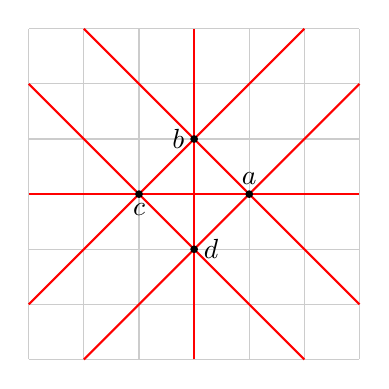
\begin{tikzpicture}[scale=0.7]
			\foreach \x in {-3,...,3} {
				\draw[black!20!white] (\x,-3) -- (\x,3);
			}
			\foreach \y in {-3,...,3} {
				\draw[black!20!white] (-3,\y) -- (3,\y);
			}
			\draw[red,thick] (-3,-2) -- (2,3);
			\draw[red,thick] (-2,-3) -- (3,2);
			\draw[red,thick] (-3,2) -- (2,-3);
			\draw[red,thick] (-2,3) -- (3,-2);
			\draw[red,thick] (-3,0) -- (3,0);
			\draw[red,thick] (0,-3) -- (0,3);
			\fill (1,0) circle (0.07) node[above]{$a$};
			\fill (-1,0) circle (0.07) node[below]{$c$};
			\fill (0,1) circle (0.07) node[left]{$b$};
			\fill (0,-1) circle (0.07) node[right]{$d$};
	\end{tikzpicture} 
	\end{center} 

	Das projektive Bild dazu, in dem sich jede Wahl von zwei der sechs Geraden einen Schnittpunkt hat. Die Schnittpunkte $ab \cap cd$ und $bc \cap ad$ haben die Form $(0 : x_1 : x_2)$ (sie befinden sich im Unendlichen). 
	\begin{center}
	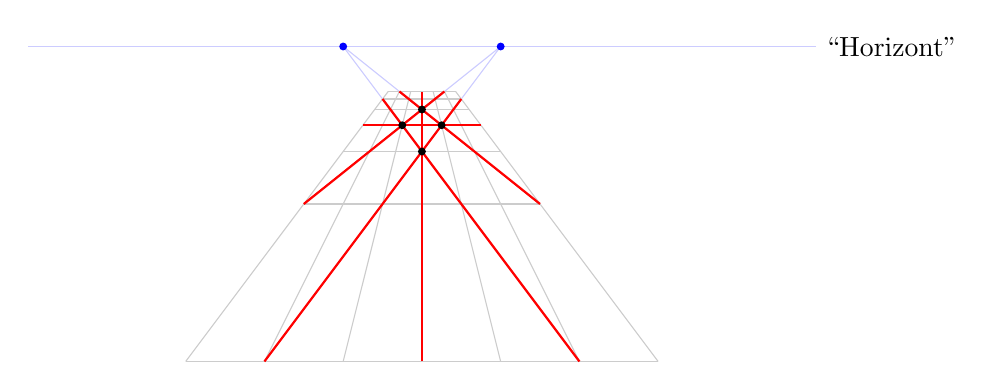
\begin{tikzpicture}
\draw[blue!20!white] (-5,1) -- (5,1) node[black,right] {``Horizont''} ;
\draw[blue!20!white] (-3/2,-1) -- (1,1);
\draw[blue!20!white] (-2,-3) -- (1,1);
\fill[blue] (1,1) circle (0.05);
\draw[blue!20!white] (3/2,-1) -- (-1,1);
\draw[blue!20!white] (2,-3) -- (-1,1);
\fill[blue] (-1,1) circle (0.05);

	\foreach \x in {-3,...,3}
{
	\draw[black!20!white] ({\x/(-3+4)},{-3/(-3+4)}) -- ({\x/(3+4)},{3/(3+4)});
}
\foreach \y in {-3,...,3}
{
	\draw[black!20!white] ({-3/(\y+4)},{\y/(\y+4)}) --  ({3/(\y+4)},{\y/(\y+4)});
}
	\foreach \xa/\ya/\xb/\yb in { -3/-2/2/3, -2/-3/3/2, -3/2/2/-3, -2/3/3/-2, -3/0/3/0, 0/-3/0/3}
{
	\draw[red,thick] ({\xa/(\ya+4)},{\ya/(\ya+4)}) -- ({\xb/(\yb+4)},{\yb/(\yb+4)});
}
	\foreach \x/\y in {1/0,0/1,-1/0,0/-1 }
{
	\fill ({\x/(\y+4)},{\y/(\y+4)}) circle (0.05);
}
	\end{tikzpicture} 
	\end{center}

Der Schnittpunkt von projektiven Geraden $ab$ und $cd$ ist $(0: -1 : 1)$. In der Sprache der Vektorräume heißt das, dass der Vektor $(0,-1,1)$ im Schnitt von $\lin( (1,1,0), (1,0,1))$ und $\lin ((1,-1,0),(1,0,-1))$ liegt. 


Der Schnittpunkt von $bc$ und $ad$ ist $(0:1:1)$.
	
\end{bsp} 

\begin{bsp}
	Im Fall vom Körper $\K = \{0,1\}$ lässt sich der projektive Raum $\bP(V)$ mit $V \setminus \{0\}$ identifizieren. Die projektive Ebene $ \K \bP^2$ für $\K= \{0,1\}$ heißt \textbf{Fano-Ebene}. Die Punkte und Geraden der Fano-Ebene können durch das folgende Diagramm: IM AUFBAU. 
\end{bsp} 
